\chapter{Background Theory}\label{chp:fundament}
\vspace{-1.5cm}
\noindent\rule{\columnwidth}{1.2mm}

%\begin{figure}[h!]
%\centering
%\caption{Regiões sensoriais e seus segmentos medulares}
%\includegraphics[width=0.91\linewidth]{Imagens/corpo.pdf}
%\label{fig:corpo}
%
%\small Fonte: \citeonline{ASIA}
%\end{figure}

\section{ROS}

There are many problems when developing robot applications, especially because the complexity of those systems. ROS is not an operating system per say, but a framework that allows coders to readily develop and test solutions with modularity and code reusability in mind. It was built in a agnostic package system that allows integration from many packages available from the ROS Open-source community, many of them implementing support libraries and proof-of-concept algorithms, as well as core infrastructure.

The main aspects of ROS are \cite{quigley2009ros}:

\begin{itemize}
\item Peer-to-peer: even though the ROS framework relies on a master or namespace as a lookup mechanism, the communication is established between peers, avoiding unnecessary routing through slow links when the recipient is on the subnet.
\item Tools-based: instead of building an intricate framework, ROS instead relies on a set of tools written to perform task, including various tools for compilation, tap data stream, data plotting, configuration, documentation generation, etc.
\item Multi-lingual: since communication between nodes relies only on XML-RPC, they can be implemented in any language, either by explicitly writing the full library that interacts with roscore or building a wrapper for the ROS C++ library.
\item Thin: many robots implementations have parts of code that could be reused in other project if they weren't so entangled with all existing code. ROS proposes an architecture where code is separated into packages that holds no dependency on ROS. All packages can be built individually using one CMake each, different from the traditional software paradigm where one CMake file builds the entire project.
\item Free and Open-source: ROS source code is publicly available and released under the BSD License, allowing copy and redistribution of the source code, including for commercial purposes.
\end{itemize}

\subsection{Packages}

In order to better build robotic system, ROS adopts a packaged architecture, making every subsystem of the application run separately from all the others. Every package can contain new nodes, libraries, configuration or even datasets.

The main advantage of this approach is making code more organized in it's own subsystems and sub-subsystems, that specialize in doing an specific task very well so that other packages can use this functionality. Packages can also be written independently of language, as long as it's supported by ROS.

\subsection{Topics}

In order for nodes to communicate, they interact publishing messages in topics. Topics are anonymous buses where each node can publish messages following the message type standards. Each node can then subscribe to topics that are relevant to them and act upon data captured on the topic. Message can even be recorded and played back to support applications that will need the information later in time.

% TODO: refazer imagem para evitar citação
\begin{figure}[!ht]
\centering
\caption{Topic initialization.}
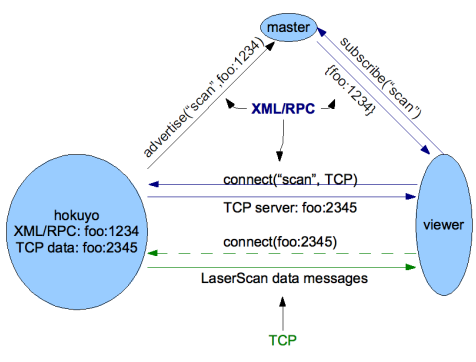
\includegraphics[width=0.5\linewidth]{rostopic}
\label{fig:rostopic}
%\small{Source: ROSWiki.}
\end{figure}

The topics are implemented in a XML-RPC protocol, using a master node in order to provide name resolution. In order for a publisher connect to a subscriber, they do the following steps:

\begin{enumerate}
\item Subscriber register with the master the topics it will be listening to.
\item Publisher register with the master the topics it will be publishing to.
\item Master informs subscriber of a new publisher.
\item Subscriber request a topic connection with the Publisher and negotiates a transport protocol.
\item Subscriber connects using the selected protocol.
\end{enumerate}

It's important to notice that, once the connection is established, the communication is maintained peer-to-peer, using former protocols like TCPROS, built over TCP/IP, and UDPROS, built over UDP. This not only provides faster communication inside the same network by not requiring the messages to be relayed through the master, but also enables communication through available networks of the Internet protocol suite, including 802.11X wireless transmission.

The topic configuration also enables true agnostic packages, since the communication between them will be done using a standardized communication medium, loosely coupling the packages and making them easily maintainable. Debugging can also be done using command-line tools that wiretap this medium and display the information exchanged by nodes.

\subsection{Services}

The topic communication can be very useful in many-to-many communication, but lacks support when sending messages or commands that require a response. When a reply is needed, it is a better practice to use services instead of topics. This is especially true for tasks that need a lot of computing power but only need to be executed once in a while, so instead of calculating it in every iteration, the service can be run just when requested and return data to the caller. The request is usually done in a similar way to Remote Procedure Calls (RPCs) in programming languages.

\subsection{Message types}

Since nodes need to understand each other, they talk following pre-defined message standards, and the message files themselves are packages that define the content of each message. To avoid confusion, each topic is initialized using a pre-defined message type and every node has to conform to it. Let's take a look at the message definition \texttt{geometry\_msgs/Twist.msg}, that is used in navigation to define linear and angular velocity for the joints:

\begin{lstlisting}
Vector3  linear
Vector3  angular
\end{lstlisting}

Note that the \texttt{Vector3} is not a base type message, but is another type of message defined at \texttt{geometry\_msgs/Vector3.msg}:

\begin{lstlisting}
float64 x
float64 y
float64 z
\end{lstlisting}

The variable types that cannot be expanded into other definitions are called primitive types. The primitive types are:

\begin{multicols}{3}
    \begin{itemize}
        \item \texttt{bool}
        \item \texttt{int8}
        \item \texttt{uint8}
        \item \texttt{int16}
        \item \texttt{uint16}
        \item \texttt{int32}
        \item \texttt{uint32}
        \item \texttt{int64}
        \item \texttt{uint64}
        \item \texttt{float32}
        \item \texttt{float64}
        \item \texttt{string}
        \item \texttt{time}
        \item \texttt{duration}
    \end{itemize}
\end{multicols}

Message types for services are done in a similar way, but since services support response, the message will consist of two individual messages. If we look at a standard definition found in \texttt{std\_srvs/SetBool.srv}:

\begin{lstlisting}
bool data
---
bool success
string message
\end{lstlisting}

This service is used for setting a boolean variable to \textit{true} or \textit{false}, that can be activating or deactivating an actuator. The response consists of a boolean that tells if the operation was successful and a message for better description in case of error.

\section{Gazebo}

Since ROS only provides the tools to develop a robot system solution, there is a need for testing the code on a real environment. In order to simulate the robot and avoid having to test every configuration on physical hardware, Gazebo provides ROS with a framework to simulate and benchmark the robot or even a group of robots accurately. The \prettyref{fig:gazebo-sim} shows the Gazebo simulation for a supported robot \cite{koenig2004design}.

\begin{figure}[!ht]
\centering
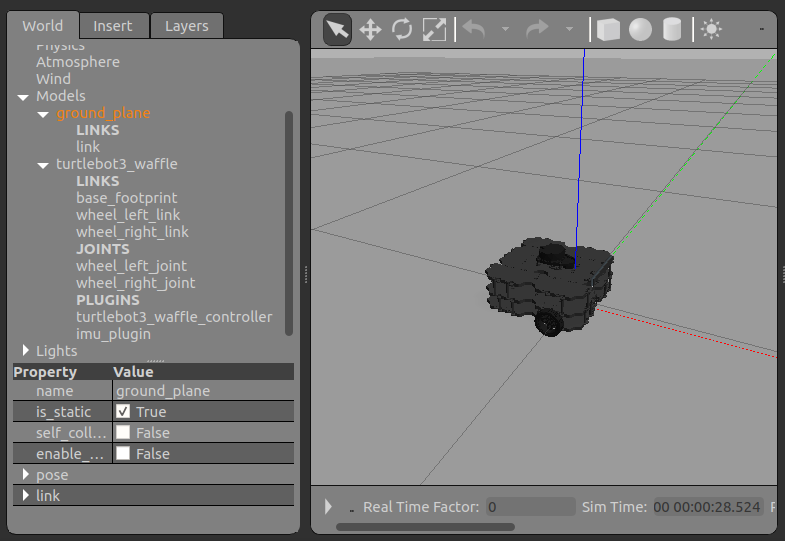
\includegraphics[width=.5\linewidth]{gazebo-sim}
\caption{Gazebo simulation suite.}
\label{fig:gazebo-sim}
\end{figure}

The Gazebo simulator offers:

\begin{itemize}
\item Dynamics Simulation using multiple physics engines.
\item Advanced 3D Graphics for high-quality rendering.
\item Sensors and Noise, to generate reliable sensor data, compatible with real-world sensors.
\item Robot Models, including ones from the community.
\end{itemize}

All the robot description is made using a URDF file or a SDF file. The URDF or Universal Robotic Description Format file is a XML file describing all elements of the robot. Even though it's called ``Universal'', it lacks some of the features like parallel linkages, friction, etc. To get around this issues, a new model called SDF or  Simulation Description Format was developed specifically for use in Gazebo, while the URDF was maintained for backward compatibility. Every time an URDF file is loaded it is converted by Gazebo to an SDF equivalent.

\subsection{URDF}

The URDF must start describing each link and it's inertia.  \prettyref{fig:gazebo-sim} show three links: \texttt{base\_footprint}, \texttt{wheel\_left\_link} and \texttt{wheel\_right\_link}. They are loaded from STL or Collada files included in the project. \prettyref{fig:gazebo-stl} show the STL renders for the robot shown on \prettyref{fig:gazebo-sim}.

\begin{figure}[!ht]
\centering
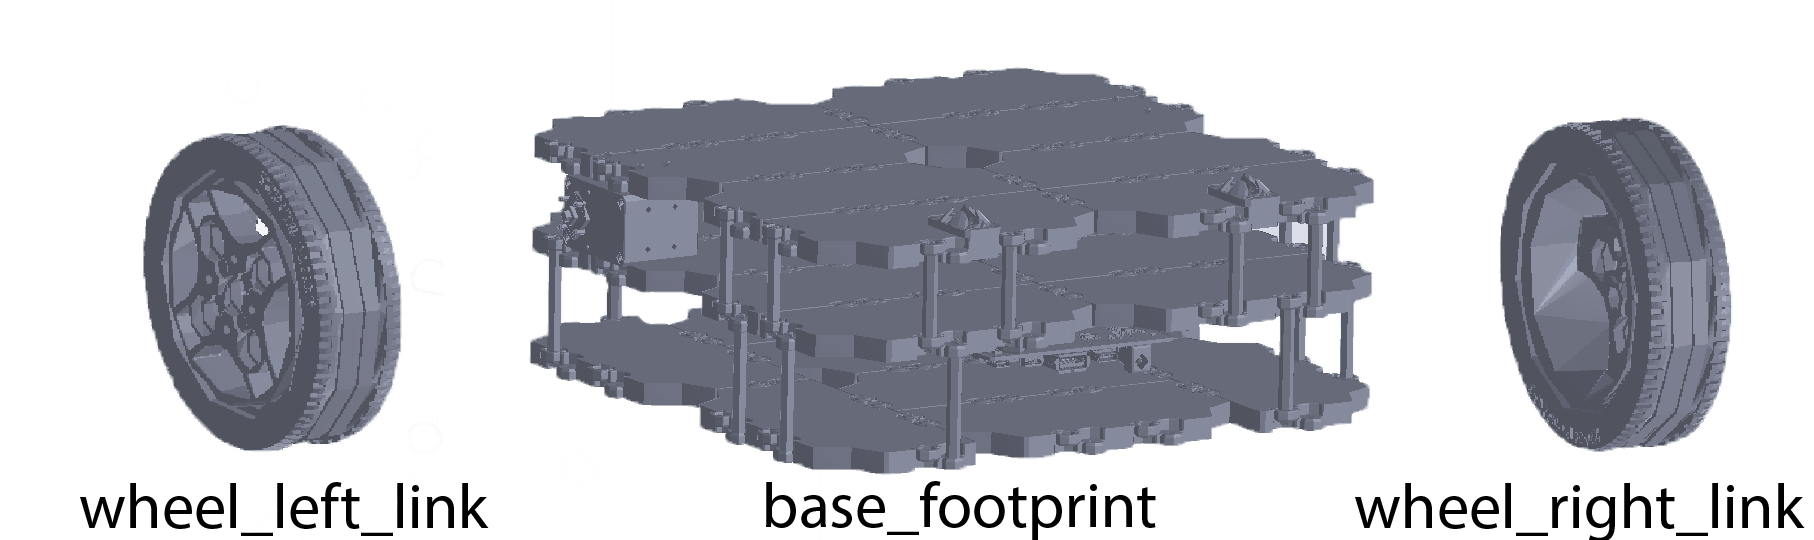
\includegraphics[width=.8\linewidth]{gazebo-stl}
\caption{STL Link files.}
\label{fig:gazebo-stl}
\end{figure}

The inertia is described by it's inertial parameters, formerly the mass, center of mass and Moment of Inertia Matrix. Additionally, you specify a collision box that will aid collision testing in simulation. You can then describe the rest of the robot, including the joints that will hold links together. Two basic joints can be seen, \texttt{wheel\_left\_joint} and \texttt{wheel\_right\_joint}, the hold all three links together. Finally, the plugins will give the robot the simulation functionality, adding IMUs, Laser Scanners, Cameras, etc.

\subsection{SDF}

The SDF is an improvement of the URDF descriptor format that supports more functionality. It not only supports all the physical descriptions shown in the URDF model, but also features:

\begin{itemize}
\item World information, from lightning and gravity to complex information like magnetic fields, winds and atmosphere (temperature and pressure).
\item Scene information, like ambient, background, sky, fog and shadows.
\item Multiple robots descriptors.
\item Choosing physics engine.
\end{itemize}

\subsection{Physics Engines}

In order to simulate the physical conditions of the robot system, Gazebo supports four different physics engines: ODE, Bullet, Simbody and DART. At the start of each simulation, the user can select the desired physics engine changing the startup flags for the program or configure it on the SDF file.

ODE or Open Dynamics Engine is an engine for simulating articulated rigid body structures. It features a stable integrator, meaning that numeric errors shouldn't grow out of control. Because of that, the simulator drops physical accuracy in favor of speed, stability and robustness \cite{smith2005open}.

Bullet is a Python implementation of physics simulation for robotics, games and visual effect that provides forward and inverse dynamics and kinematics, as well as built in collision detection. Bullet differentiates itself by being easy to use and provide integration to machine learning frameworks like TensorFlow \cite{coumans2018}.

Simbody is a multibody simulator focused on biomedical research. It was developed to better suit simulation scenarios where engines like ODE may not converge to correct results because of lack of fidelity in favor of real-time performance. It is used for neuromuscular, prosthetic, and biomolecular simulation, as well as design and control of humanoid robots \cite{sherman2011simbody}.

DART or Dynamic Animation and Robotics Toolkit is another rigid body simulation that distinguishes itself by accuracy and stability. The main purpose of this simulator is providing full access to internal kinematic and dynamic quantities \cite{lee2018dart}.

\subsection{Simulation}



\subsection{Sensors and actuators}

%\section{OpenCV}

%\section{MoveIT!}

\section{COB}

The Care-o-bot is a project for a mobile assistive robot that is modular, developed and maintained by Fraunhofer IPA. The COB version 4 can be seen on \prettyref{fig:cob4}. The robot was composed not only to provide researchers a reliable mobile base, but also to aid research on human-robot interaction and social behavior \cite{mci/Kittmann2015}. It is composed mainly by a mobile base, a torso and a head.

% TODO: editar a imagem para conter descrição de partes
\begin{figure}[!ht]
\centering
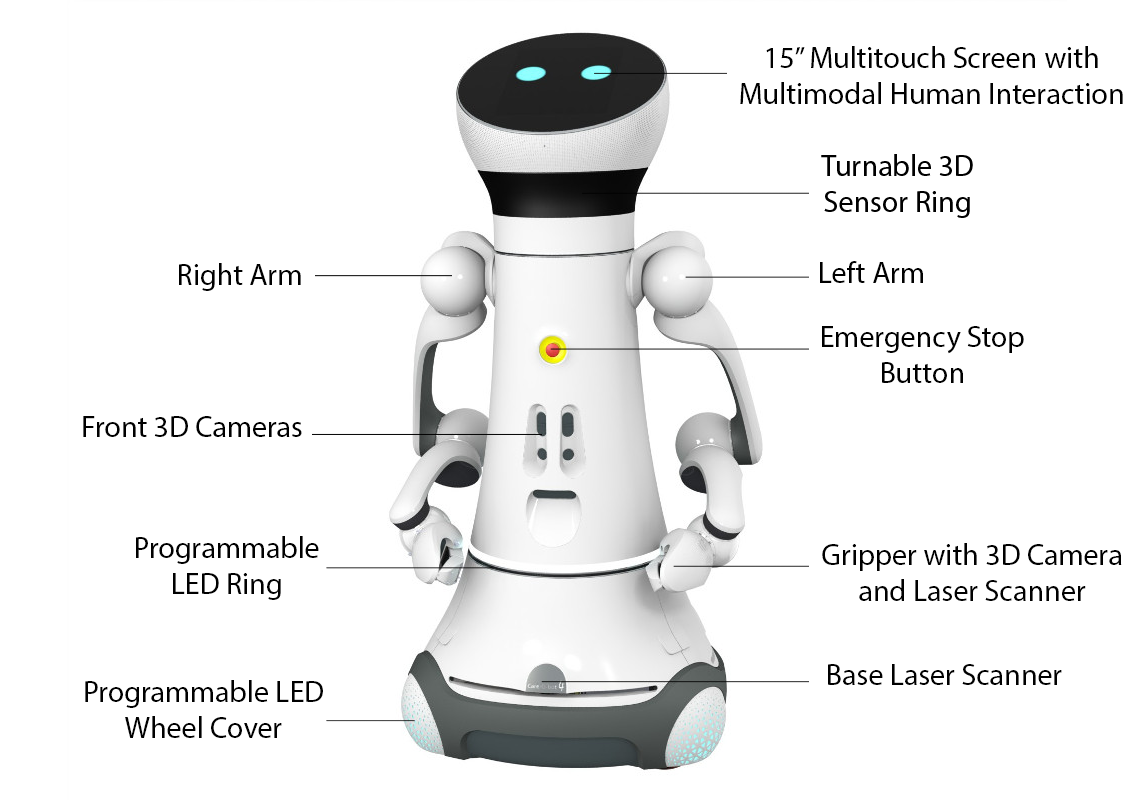
\includegraphics[width=.8\linewidth]{cob4}
\caption{COB 4 full robot with both manipulators.}
\label{fig:cob4}
\end{figure}

\subsection{Base}

The base features three steerable wheels used for moving the robot on the ground. The wheels can rotate on the vertical axis, allowing movement in every direction. It is also equipped with 2D laser scanners for object detection and safety, the battery for the robot and the control panel.

\subsection{Torso}

The torso is linked with the base using a spherical joint, providing 3DOF, cameras, a LED Ring, two optional arms with 7DOF each, with a manipulator finger with 2DOF. The manipulator also has cameras and laser scanner for object recognition and picking.

\subsection{Head}

The head is linked with torso also with a spherical joint, and contain the human interface to interact with user, including the sound system, microphone, a touch screen display and optional camera for face recognition.


\subsection{Package organization}

The COB is built around ROS and includes a different sets of packages for different purposes. Since the robot support different configurations (manipulators, joints, mobile bases), some packages are optional. \prettyref{fig:dependency-graph} shows the dependency graph for the first three layers of packages. Notice that the arrangement is quite intricate even showing only the packages written exclusively for COB (not showing other ROS packages used on COB).

\begin{figure}[!ht]
\centering
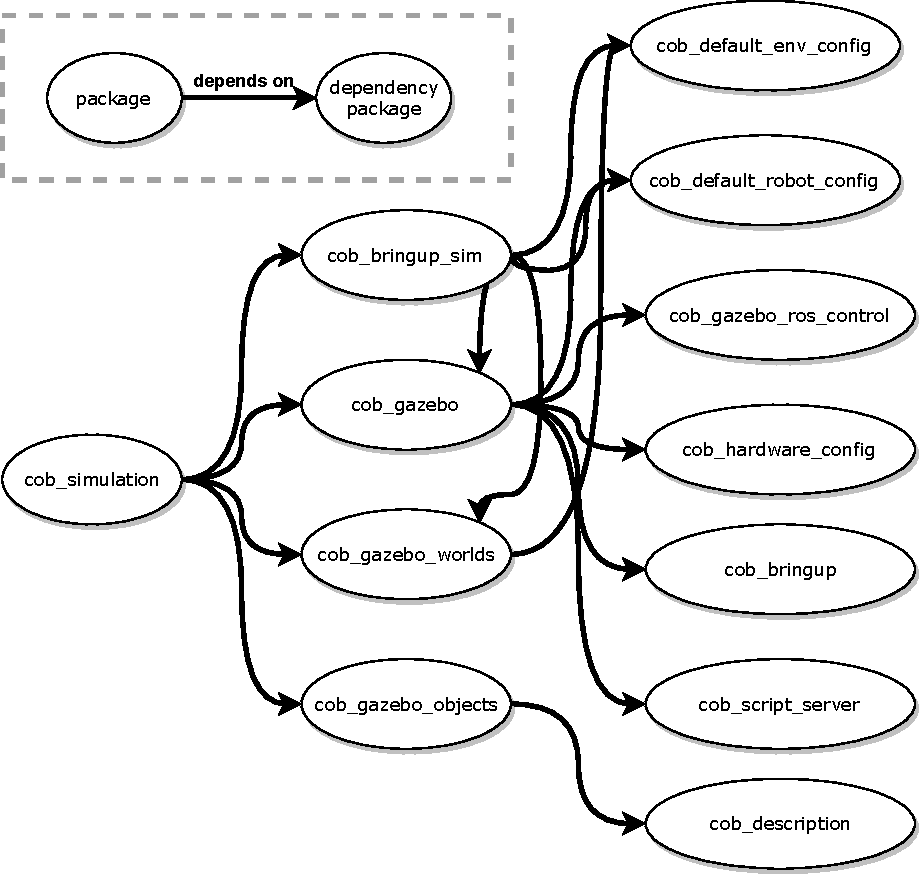
\includegraphics[width=.7\linewidth]{dependency-graph}
\caption{Dependency graph of \texttt{cob\_simulation} with depth 3.}
\label{fig:dependency-graph}
\end{figure}


The COB core consist of the following packages and its dependencies:

\begin{itemize}
\item \texttt{cob\_msgs}: Robot-specific Messages, representing state information like battery status, etc.
\item \texttt{cob\_srvs}: Robot-specific Services.
\item \texttt{cob\_description}: Robot URDF models different COB configurations (only base, base with fixed torso, base with actuated torso, etc).
\item \texttt{cob\_bringup}: machine configuration, including all scripts and dependencies required to run COB.
\end{itemize}

COB also features high-level capabilities, some of them being:

\begin{itemize}
\item \texttt{cob\_command\_tools}: high-level utilities command tools, including API for commonly used movements, control dashboard, teleoperation and status monitoring.
\item \texttt{cob\_driver}: plugins interfacing motors, LEDs, sound system, cameras, batteries and even the facial expressions for the robot, and providing their data in the form of topics and services.
\item \texttt{cob\_navigation}: provides tools for robot navigation, including creation of maps, navigation with/without collision avoidance and navigation in dynamic environments.
\item \texttt{cob\_object\_perception}, \texttt{cob\_people\_perception}, \texttt{cob\_environment\_perception}: computer vision libraries used for perception of the environment.
\item \texttt{cob\_manipulation}: manipulator related package, including inverse kinematics, arm motion planning and collision avoidance.
\end{itemize}



\subsection{Basic components}

